\documentclass{beamer}
\usepackage[utf8x]{inputenc}
\usepackage[ngerman]{babel}
\usepackage{amsmath}
\usepackage{amsfonts}
\usepackage{amssymb}
\usepackage{graphicx}
\usepackage{subfigure}
\author{Johannes Hackel und Falco Prescher}
\title{Bildverarbeitung mit OpenCL}

\usetheme{Ilmenau}
\useoutertheme{split}
\usecolortheme{rose}

\newcommand*\oldmacro{}%
\let\oldmacro\insertshorttitle%
\renewcommand*\insertshorttitle{%
  \oldmacro\hfill%
  \insertframenumber\,/\,\inserttotalframenumber}

\begin{document}

\begin{frame}
\titlepage
\end{frame}

\begin{frame}
\frametitle{Bildverarbeitung mit OpenCL}
\tableofcontents
\end{frame}

\section{OpenCL}

\subsection{Allgemeines zu OpenCL}
\begin{frame}
\frametitle{Allgemeines zu OpenCL}
\begin{itemize}
\item Test
\end{itemize}
\end{frame}

\subsection{Kernelverteilung unter Devices und Command Queue}

\subsubsection*{Kernelverteilung unter Devices}
\begin{frame}
\frametitle{Kernelverteilung unter Devices}
\begin{figure}
\begin{center}
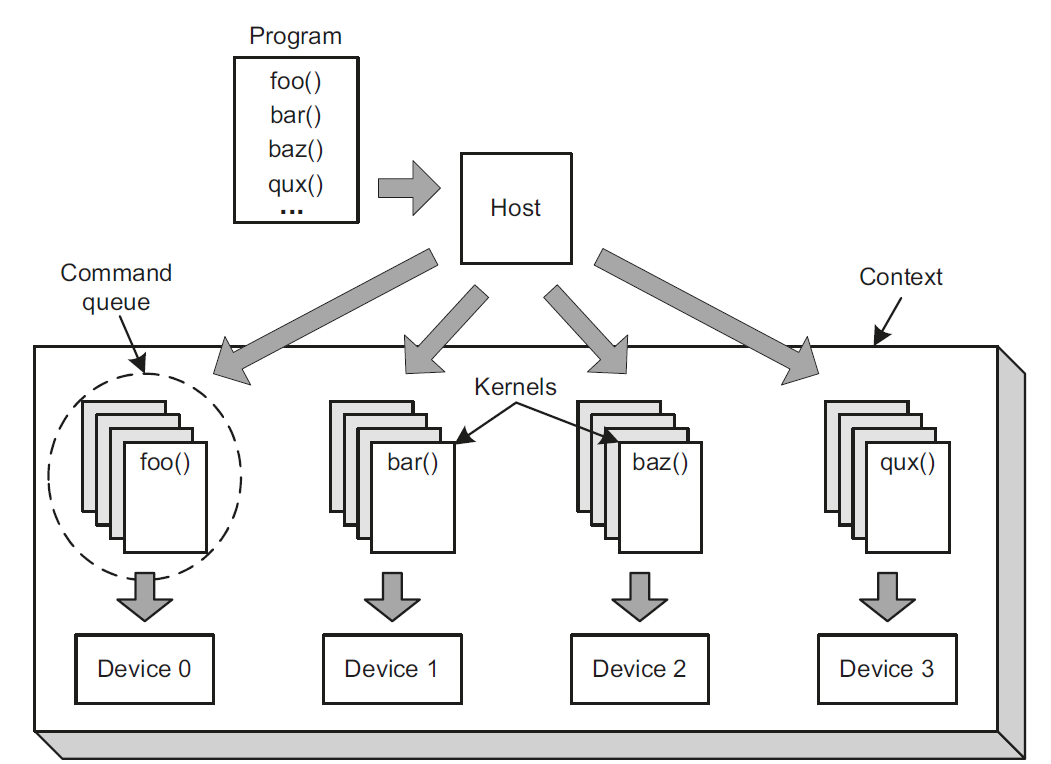
\includegraphics[width=8cm]{kernel_distr_manning_p8.PNG}
\footnote{\tiny{Scarpino Matthew: OpenCL In Action, \\Manning Publications Co., 2012, S. 8}}
\end{center}
\end{figure}
\end{frame}

\subsubsection*{Command Queue}
\begin{frame}
\frametitle{Command Queue}
\begin{figure}
\begin{center}
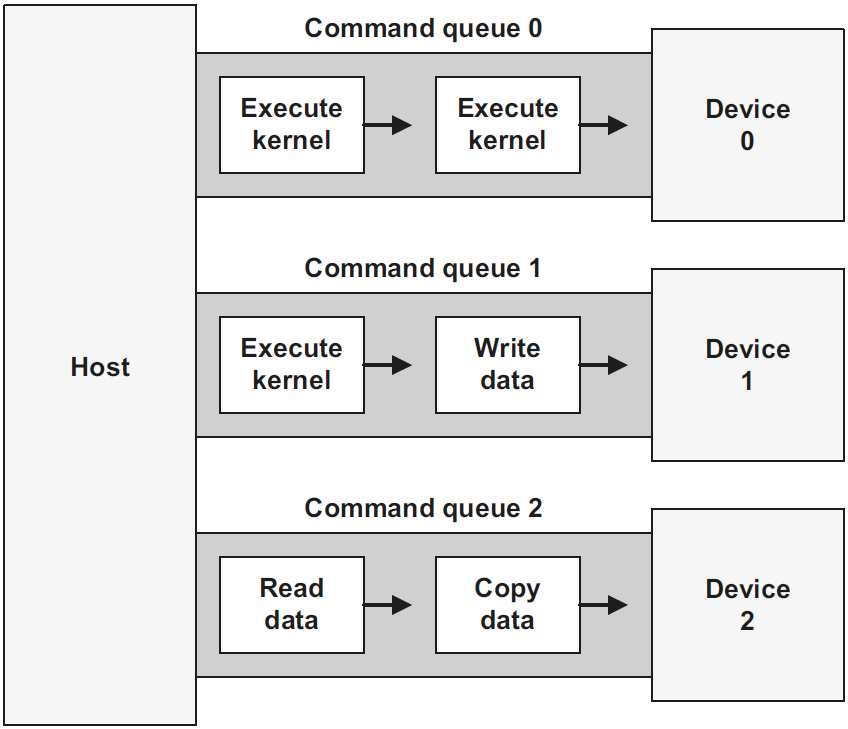
\includegraphics[width=6cm]{command_queue_manning_p39.PNG}
\footnote{\tiny{Scarpino Matthew: OpenCL In Action, \\Manning Publications Co., 2012, S. 39}}
\end{center}
\end{figure}
\end{frame}

\subsection{Workgroups und Compute Units und Device Model}

\subsubsection*{Workgroups und Compute Units}
\begin{frame}
\frametitle{Workgroups und Compute Units}
\begin{figure}
\begin{center}
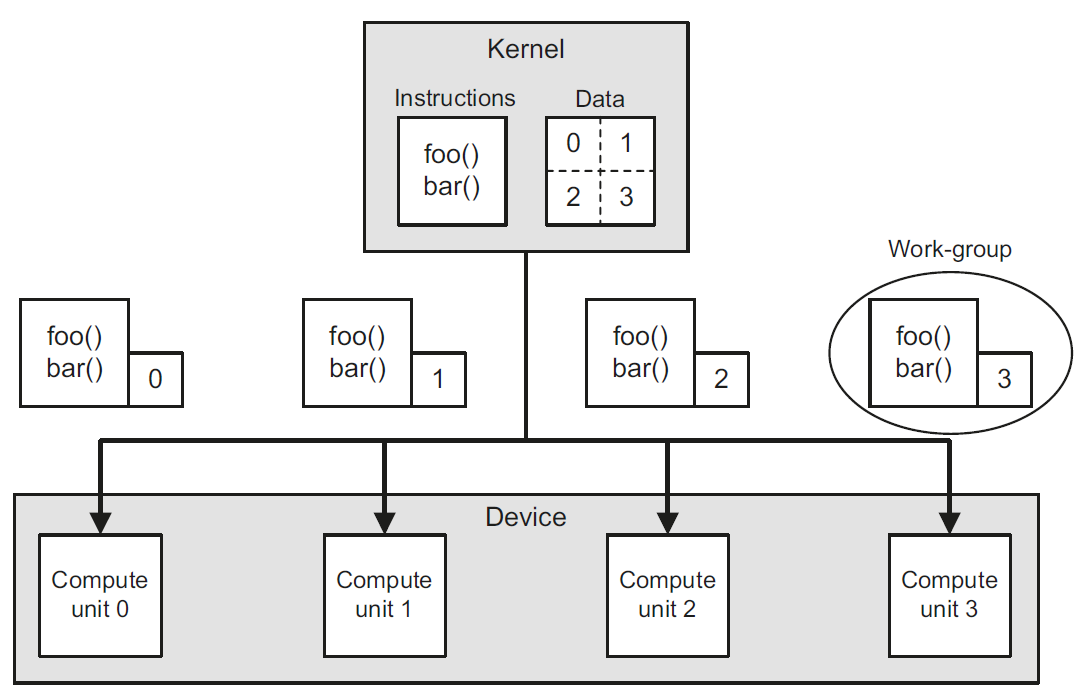
\includegraphics[width=8cm]{workgroups_to_compute_units_manning_p66.PNG}
\footnote{\tiny{Scarpino Matthew: OpenCL In Action, \\Manning Publications Co., 2012, S. 66}}
\end{center}
\end{figure}
\end{frame}

\subsubsection*{Device Model}
\begin{frame}
\frametitle{Device Model}
\begin{figure}
\begin{center}
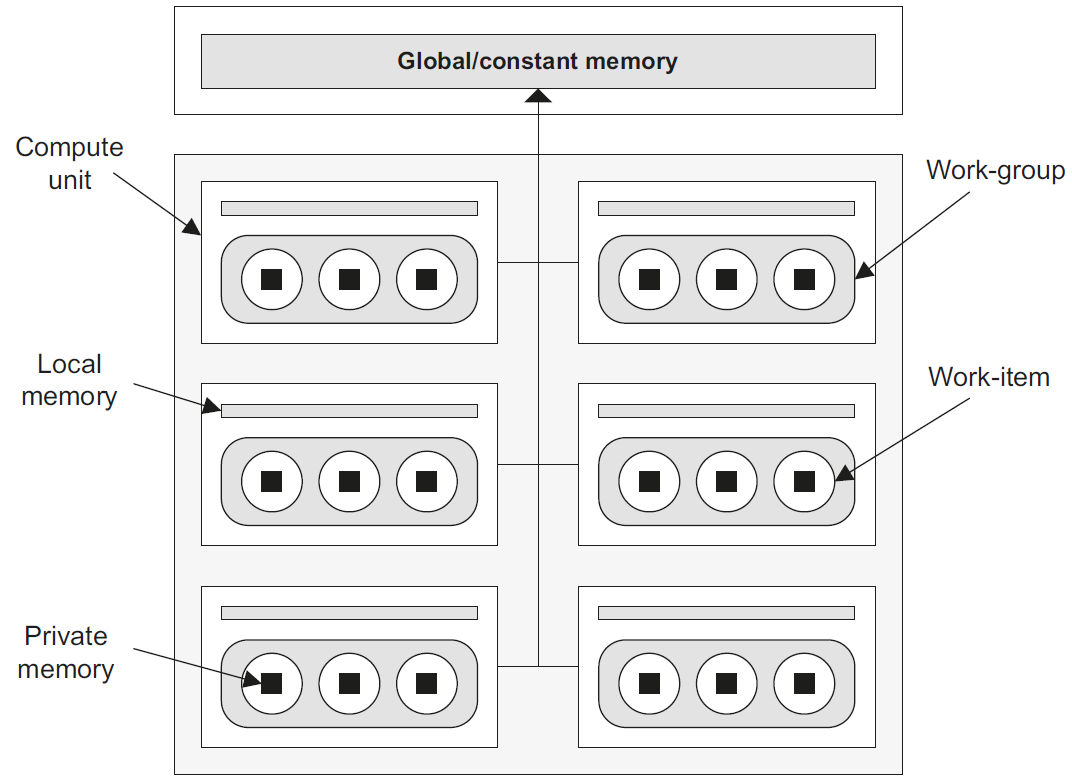
\includegraphics[width=8cm]{device_model_manning_p87.PNG}
\footnote{\tiny{Scarpino Matthew: OpenCL In Action, \\Manning Publications Co., 2012, S. 87}}
\end{center}
\end{figure}
\end{frame}

\subsection{Events in OpenCL}

\subsubsection*{Wait Lists}
\begin{frame}
\frametitle{Wait Lists}
\begin{figure}
\begin{center}
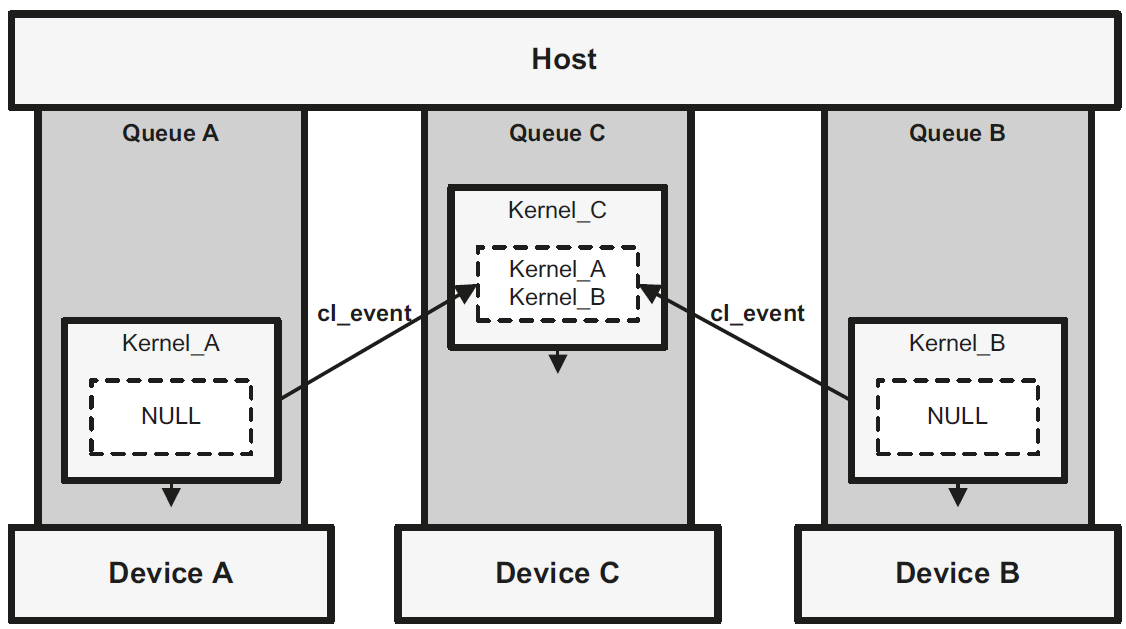
\includegraphics[width=9cm]{wait_lists_command_sync_p146.PNG}
\footnote{\tiny{Scarpino Matthew: OpenCL In Action, \\Manning Publications Co., 2012, S. 146}}
\end{center}
\end{figure}
\end{frame}

\subsubsection*{Wait Command}
\begin{frame}
\frametitle{Wait Command}
\begin{figure}
\begin{center}
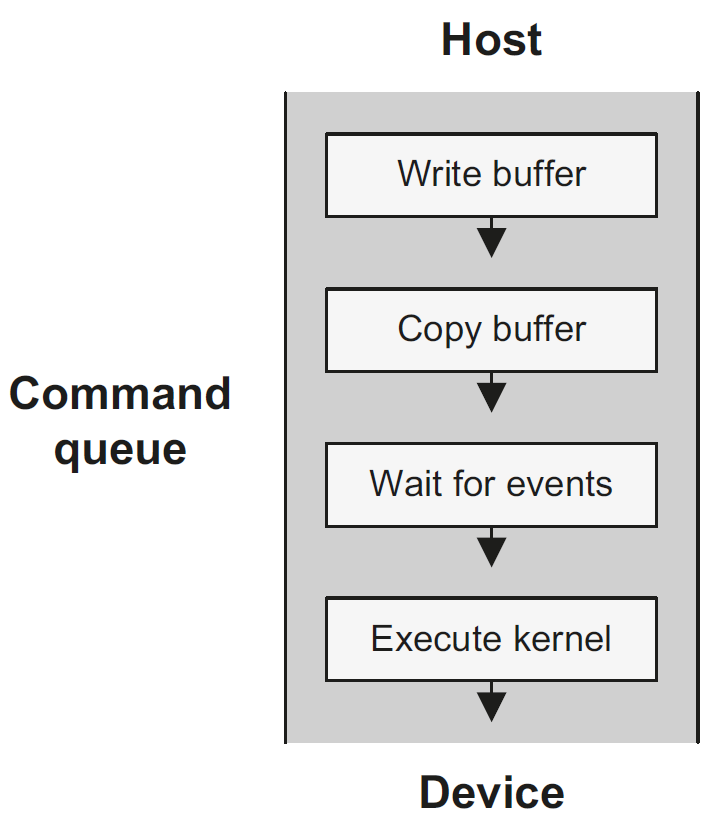
\includegraphics[width=5cm]{wait_command_p150.PNG}
\footnote{\tiny{Scarpino Matthew: OpenCL In Action, \\Manning Publications Co., 2012, S. 150}}
\end{center}
\end{figure}
\end{frame}

\section{Vergleich von OpenCL mit CUDA}

\subsection{Unterstütze Plattformen}
\begin{frame}
\frametitle{Unterstütze Plattformen}
CUDA:
\begin{itemize}
\item NVIDIA-GPUs
\newline
\end{itemize}
OpenCL:
\begin{itemize}
\item alle Recheneinheiten die OpenCL unterstützt
\item CPUs, GPUs
\end{itemize}
\end{frame}

\subsection{Performance}
\begin{frame}
\frametitle{Performance}
CUDA:
\begin{itemize}
\item Hardware und Technologie vom gleichen Hersteller
\item gute Implementation
\item gute Leistung
\newline
\end{itemize}
OpenCL:
\begin{itemize}
\item von Plattform abhängig
\item Faktoren: Leistung, Implementation
\end{itemize}
\end{frame}

\subsection{API/Modell}
\begin{frame}
\begin{center}
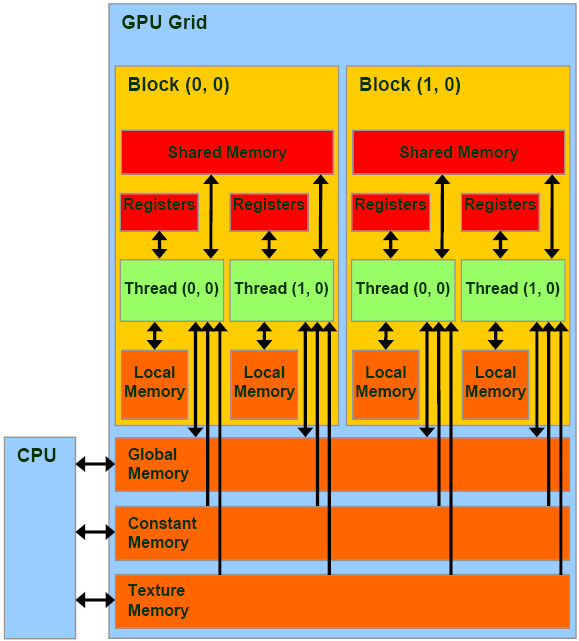
\includegraphics[width=6cm]{CUDAmodel.png}
\footnote{\tiny{CUDA Modell,  Quelle: [2]}}
\end{center}
\end{frame}

\begin{frame}
\frametitle{API/Modell}
\begin{itemize}
\item Modelle ähneln sich
\item Begriffsunterschiede
\item weitere Unterschiede in der Syntax
\end{itemize}
\end{frame}

\begin{frame}
\begin{center}
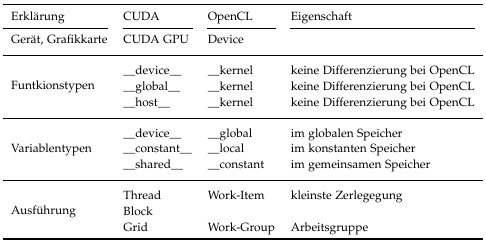
\includegraphics[width=10cm]{cuda_opencl_begriffe.png}
\footnote{\tiny{Quelle: [2]}}
\end{center}
\end{frame}

\subsection{Entwicklungsaufwand}
\begin{frame}
\begin{center}
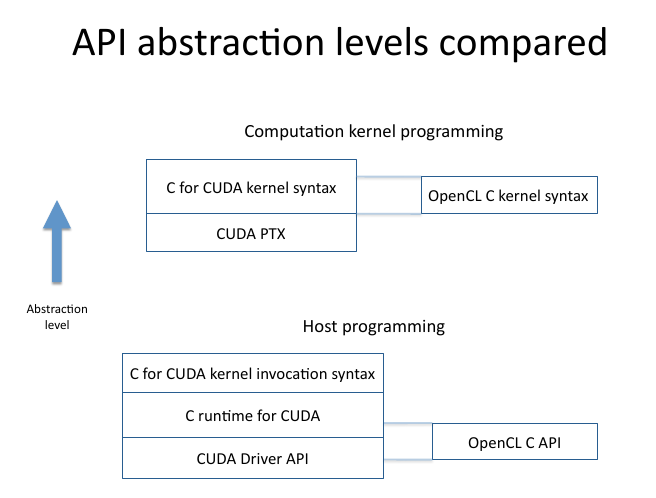
\includegraphics[width=9cm]{api_abstraction_level.png}
\footnote{\tiny{Quelle: [3]}}
\end{center}
\end{frame}

\begin{frame}
\frametitle{Entwicklungsaufwand}
OpenCL:
\begin{itemize}
\item API mit geringer Abstraktion
\item verschiedene Debugging-Möglichkeiten je Plattform
\item guter Debugger(cross-plattform): gDEBugger
\item verschieden Geräte: unterschiedliche Implementation
\newline
\end{itemize}
CUDA:
\begin{itemize}
\item geringe und hohe Abstraktion
\item viele Bibliotheken
\item guter Debugger durch CUDA-SDK
\end{itemize}
\end{frame}

\subsubsection*{Fazit}
\begin{frame}
\frametitle{Fazit}
$\to$
für High-Performance-Cluster mit gleicher Hardware und speziell angefertigter Software
\newline
$\Rightarrow$
CUDA zu bevorzugen
\newline
\newline
$\to$
im Consumerbereich bei Verwendung von verschiedener Hardware
\newline
$\Rightarrow$
OpenCL bevorzugt
\end{frame}

\section{Bildverarbeitung}

\subsection{Allgemeines zu Bildverarbeitung mit OpenCL}
\begin{frame}
\frametitle{Allgemeines zu Bildverarbeitung mit OpenCL}
\begin{itemize}
\item spezielle Datentypen (image2d\_t, image3d\_t) und Funktionen im OpenCL C
\item Image2D und Image3D Klassen in der C++ API
\item Verschiedene Datentypen für Channels
\item Verschiedene Reihenfolge der Channels
\item maximale Größe eines Images je Plattform festgelegt
\end{itemize}
\end{frame}

\subsection{Kantenerkennung in Bildern}
\begin{frame}
\frametitle{Kantenerkennung in Bildern}
Ablauf:
\begin{enumerate}
\item Graubild erstellen und entrauschen
\item Anwendung des Sobeloperators je Pixel in X-Richtung und Y-Richtung mit den Nachbarwerten
\item Kombination beider Ergebnisse ergibt Kantenwert des Pixels
\end{enumerate}
\end{frame}

\subsubsection*{Kantenerkennung in Bildern mit OpenCL}
\begin{frame}
\frametitle{Kantenerkennung in Bildern mit OpenCL}
Verwendeter einfacher Algorithmus:
\begin{enumerate}
\item Differenzen der gegenüberliegenden Pixel
\item der höchste Wert wird der Kantenwert des Pixels
\end{enumerate}
\end{frame}

\begin{appendix}
\begin{frame}
\frametitle{Quellen}
\begin{enumerate}
\item Scarpino Matthew: OpenCL In Action, \\Manning Publications Co., 2012
\item \url{ftp://ftp.informatik.uni-stuttgart.de/pub/library/medoc.ustuttgart_fi/DIP-3178/DIP-3178.pdf}
\item \url{https://wiki.aalto.fi/download/attachments/40025977/Cuda+and+OpenCL+API+comparison_presented.pdf}
\end{enumerate}
\end{frame}
\end{appendix}

\end{document}
